\section{Summary}

A paper entitled “Vision Based Guidance for Robot Navigation in Agriculture” was based on a study conducted on Australia. Here, they had an implementation of a vision-based texture tracking method to guide autonomous vehicles in agricultural fields. While it imposed a challenging task to detect crop rows, existing methods require visual difference between what crop is against what soil is for visual segmentation. Their proposed method involves extracting and tracking the direction and offset that existed among parallel textures in a simulated overhead view of the scene. Also, they allowed neglecting of crop-specific details such as color, spacing and periodicity. The results explained the demonstration of the method in both day and night times to autonomously guide a robot across crop rows.
 
    An abridged, proposed algorithm design was as follows
\begin{itemize}
\item Pre-processing the image to correct lens distortion and to downsample the image for better processing speed\item Using an Inertia Management Unit to detect the horizon
\item Warping the stabilized image into an overhead view
\item Estimating the vehicle’s heading with respect to the crop rows thru estimation of a dominant parallel texture in the overhead image
\item Correcting heading in the overhead view via image-skewing from the estimated heading
\item Generating a frame template thru the summation of the columns found on the skewed images
\item Assuming a lateral motion that was relative to the crop by comparing such template to an initial crop template
\end{itemize}
\tab Notably citing the Horizon Detection, the researchers began to track the horizon via selecting an image region (free of obstruction from a clear horizon view) within three standard deviations of estimated horizon position. In turn, the pixels were classified into as sky or ground. Further, they also had the estimation of the row direction. Their method was to sum skewed images from varying angles along the columns then calculating the variance of the resulting vector. The skew angle with the greatest variance was the best estimate to qualify as the heading angle. Finally mentioning the detection of rows, their study contained the instance on which the field did not have any crop rows to track (e.g. the ends of the field were bare patches). In these situations, they examined the output of the summation of skewed images aforementioned. They set a standard of frame templates that vary from +/- 30 degrees.
 
Another paper entitled “Video Streaming In Autonomous Mobile Robot Using Wi-Fi” was used to consider the relevance of a capable telemetry system. Having an autonomous mobile robot required to cover a distance from one point to another with two or more wheels. To reach a destination, it was not always possible that a person could not reach. Through an Autonomous Arduino Yun for four-wheeled mobile robots, it gave capabilities to robots to actually move from one point to another by finding paths and avoiding obstacles thru Video Streaming. Achieved thru Wi-Fi Technology (as avoidance to using Bluetooth technology due to its lesser security and shortness of range), the best path was identified thru Aggrandized Genetic Algorithm (AGA) which was comparatively greater than other algorithms. Wi-Fi (IEEE 802.11 b/g/n) was used to achieve secure communications at long distances.
 
Upon mentioning Arduino Yun, it was one of the many boards and kits that Arduino sell to their users. Weighing 32 grams with lateral dimensions of 73 millimeters by 53 millimeters, Arduino Yun was usually used for Wi-Fi technology; due to its in-built Wi-Fi (IEEE 802.11 b/g/n). Along with this, this board supported USB port, MicroSD card Slot, three reset buttons, In-circuit Serial Programming header, 16MHz Crystal Oscillator, 20 Digital Input and Output Pins and 12 Analog Channels. Concentrating more on the aspect of video streaming, the Arduino Yun was capable of capturing video data to an SD card. Hence, in order to facilitate teleportation that indicated two types of operation where a machine was set to a distance: automatic mode and manual mode. The former allowed the Arduino board to send Wi-Fi standard control signals in high data rate and good quality, uninterrupted video transmission. The latter allowed recorded data to be extracted from the SD card.
 
The study entitled “Camera-Based Clear Path Detection” used to detect clarity of paths as driver assistance towards obstacle avoidance on roads. With the assumptions made of video camera calibration and vehicle information (vehicle speed and yaw angle) were known, the researchers generated perspective patches for feature extraction in the image. Then, an initial estimate of the probability of a clear path is determined thru a support vector machine (SVM). With this, they performed probabilistic patch smoothing based on spatial and temporal constraints to improve estimates.
 
    What was notable to this study was the perspective patch generation. Of which, the traditional way of determining objects without considering perspective information are fixed-grid patch and dynamic-size patch. Since objects were found to be perpendicular to the camera’s optical axis, the clear path lied on the ground and was parallel to the camera’s optical axis. Instead of defining patches in image coordinates, they referenced the patches according to world coordinates that were lying on the ground.
   
    A paper entitled “An Efficient Crop Row Detection Method for Agriculture Robots” was used to develop an efficient crop row detection method on a vision-based navigation for agriculture robots. The researchers proposed no low-level features (such as edges and middle lines found on images) were needed. Therefore, complex algorithms for edging and matching (especially the Hough transform) were avoided. This enabled conservation of computation loads. Further, a flexible quadrangle was defined to detect crop rows, where it extended or shrank this quadrangle to localize the crop rows from captured frames. The study demonstrated that this method was proven effective with high time efficiency and detection accuracy.
 
    Involving this study was the image pre-processing. Two methods, as existent in the paper, pertained to this pre-processing: Full-color images to gray-level images and Binarization. The former was used to create convenience. But, the issue of preventing loss of information happened when colors were devoid. And, it was a very common practice to convert full-color images to grayscale ones. In agriculture applications, crops and/or weeds are taken into account. With the background soil as reference, plants that belong to the green chromatic coordinate, was referred to outline such component while depressing that of the soil’s. Therefore, it made it easier to isolate these from the background. Following, binarization was key to object-recognition and tracing applications. Under grayscale conditions, this method was highly used to isolate objects from the background. All the while, it was critical to consider thresholds. These might had lead to significant impact on the binary image quality and computation loads. A method was proposed to choose the threshold thru minimizing the intra-class variance of black and white pixels; which was widely used in image-processing called Otsu’s Threshold.
 
    The highlight of the study was about the flexible quadrangle. The method implied the localization of crop rows without the need of edging or line fitting. The left and right boundarie of the quadrangle were split into four sections shown in the figure below. Each boundary box had a width of one pixel. These boxes were modified of their positions during the vehicle’s proceeding to assure that the quadrangle tightly locked the crop row through Hough Transforms. In essence, the whole gist of their proposed method were as follows:
    \begin{itemize}
\item Initializing quadrangles. From the very first image, the quadrangle positions and dimensions were given by other methods or as manually indicated in the paper.
\item Pre-processing of image. While the vehicle moved, it was obtained of the grey scaling image via 2G-R-B colour space and binarizing the grey scaling image using Otsu’s threshold at every image fed.
\item Check the hitting and mishitting conditions of the boundary boxes.
\item Modify the position of boundary boxes.
\item For the following image, keep the boundary box positions and dimensions and repeat from second bullet.
\end{itemize}

A paper from Iran entitled “A technical review on navigation systems of agricultural autonomous off-road vehicles” was used to evaluate the navigation systems for autonomous vehicles used for agriculture. The predicament on the paper was that the man-power on agriculture were decreased as industries attracted these labor force away. As a solution, researchers on this paper were to design navigation systems for autonomous off-road vehicles. In order for the navigation system to work, multiple sensors were considered. Some of it were Machine Vision, Real Time Kinetic-Global Positioning, Mechanical Sensors, Inertial Sensors Geomagnetic Direction Sensor (GDS), Ultrasonic, Fiber Optic Gyroscope (FOG), Laser Radar (LADAR), Light Detection And Ranging (LIDAR), Optical encoder, Potentiometer, Radio Frequency receiver (RF receiver), Piezoelectric yaw rate sensor, Near Infra-Red (NIR), and Acoustic sensor. These sensors are the initial element in controlling the autonomous vehicle. Fig.~\ref{fig:con} shows the Block Control Diagram of autonomous vehicles.

\begin{figure}[!h]
	\centering
	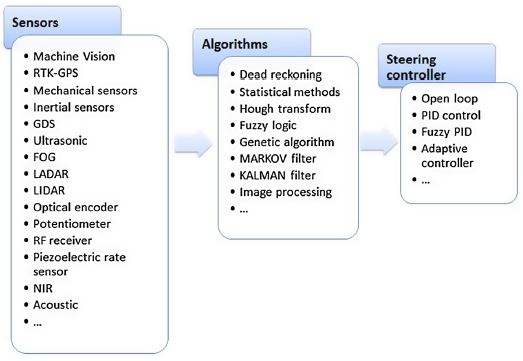
\includegraphics[width=3.5in]{control}
	\caption{Basic control diagram of autonomous vehicles.}
	\label{fig:con}
\end{figure}

In North America, the study “Agricultural automatic guidance research in North America” was published. It was established that Agricultural-related guidance research in North America has been review. Sensing Technologies were utilized and it was combined for automatic guidance. Automation depends on the ability of the researchers to maximize the performance of systems. Fig.~\ref{fig:elemen} shows the basic elements of agricultural vehicle automation systems.

\begin{figure}[!h]
	\centering
	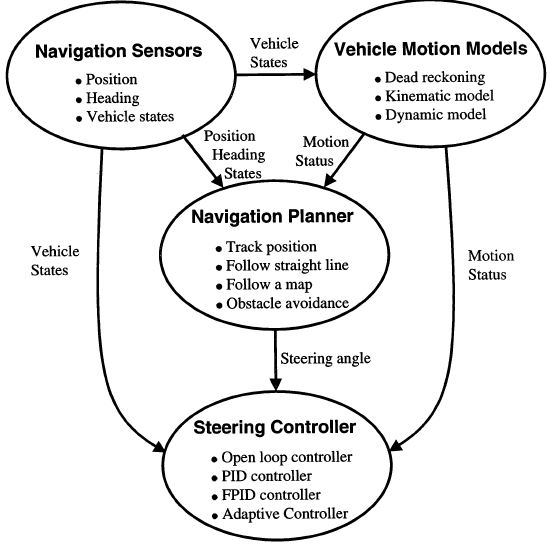
\includegraphics[width=3.5in]{elemen}
	\caption{Basic elements of agricultural vehicle automation systems}
	\label{fig:elemen}
\end{figure}

A similar study was implemented in Germany with the title “Automatic guidance for agricultural vehicles in Europe” was published. This paper focused on the automatic guidance of automatic agricultural vehicles. Different types of sensor and machine vision were used to implement the study. In line with the machine vision fragment, the row arrangement of crops were significantly considered in the development of the vehicle that utilizes machine vision. Fig.~\ref{fig:digit} shows the images related to the field tests performed. The image was digitized and guidelines were added.

\begin{figure}[!h]
	\centering
	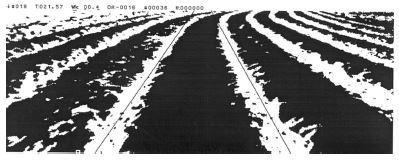
\includegraphics[width=3.5in]{digit}
	\caption{Digitised image with guidelines.}
	\label{fig:digit}
\end{figure}

One research is about the autonomous agriculture vehicles in Japan. This research has been developed in universities and government institutes, and by agricultural machinery manufacturers. The research wasn’t able to push through the whole research in the universities due to funding limitations, because of this research in universities has concentrated on methodologies, such as navigation, sensing, and application of control theory. Development of a one dimensional image sensor, and application of neural networks and genetic algorithms, has taken place at Hokkaido University; vision guidance and fuzzy logic application at the University of Tokyo; an automatic follow-up vehicle has been developed at Kyoto University; and an automatic transport vehicle at Ehime University. At research institutes and manufacturers, with their greater financial freedom, more practical systems have been developed. A tilling robot and a driver-less air blast sprayer is being developed in the Bio-oriented Technology Research Advancement Institute (BRAIN); and an autonomous rice planter, a tillage robot and autonomous forage tractor in the research institute of the Ministry of Agriculture, Forestry, and Fishery (MAFF). Kubota Co. Ltd has developed autonomous rice planting and husbandry vehicles. 

Another research is about the variable field-of-view machine vision based row guidance of agricultural robot. A new variable field-of-view machine vision method was developed allowing an agricultural robot to navigate between rows in cornfields. The machine vision hardware consisted of a camera with pitch and yaw motion control. Guidance lines were detected using an image-processing algorithm, employing morphological features in a far, near and lateral field of view, and the robot was guided along these lines using fuzzy logic control. The vehicle that they tested successfully traveled through a distance of 30 m towards the end of a crop row in three replications. 

Another article discusses the navigation system for agricultural machines. This article presents a new kind of navigation system for agricultural machines. The focus is on trajectory control where a Nonlinear Model Predictive path tracking for tractor and trailer system is presented. The experiments of the proposed method are carried out by using real agricultural machines in real environments. The goal of the research was to build a system, which is able to have at least the same accuracy as a human driver. The sufficient accuracy requirement was at most 10 cm lateral error at a speed of 12 km/h. The results presented in the article show that the goal was met and NMPC is a feasible method for accurate path tracking. 



